\documentclass{beamer}

\usepackage{graphicx}
\usepackage{amsmath}
\usepackage{physics}


\usetheme{metropolis}

\title {Spacetime Algebra}
\author {Cocoa}
\date{\today}
\institute{Ashoka University}

\graphicspath{{./Figures/}}

\begin{document}
\maketitle
	
\begin{frame}{Table of contents}
	\setbeamertemplate{section in toc}[sections numbered]
	\tableofcontents[hideallsubsections]
\end{frame}

\section{Geometric Algebra}

\begin{frame}{The Physical Problem}

Physical quantities such as angular momentum and electromagnetic fields should be invariant under parity inversion. 
\pause

\begin{figure}
	\centering
	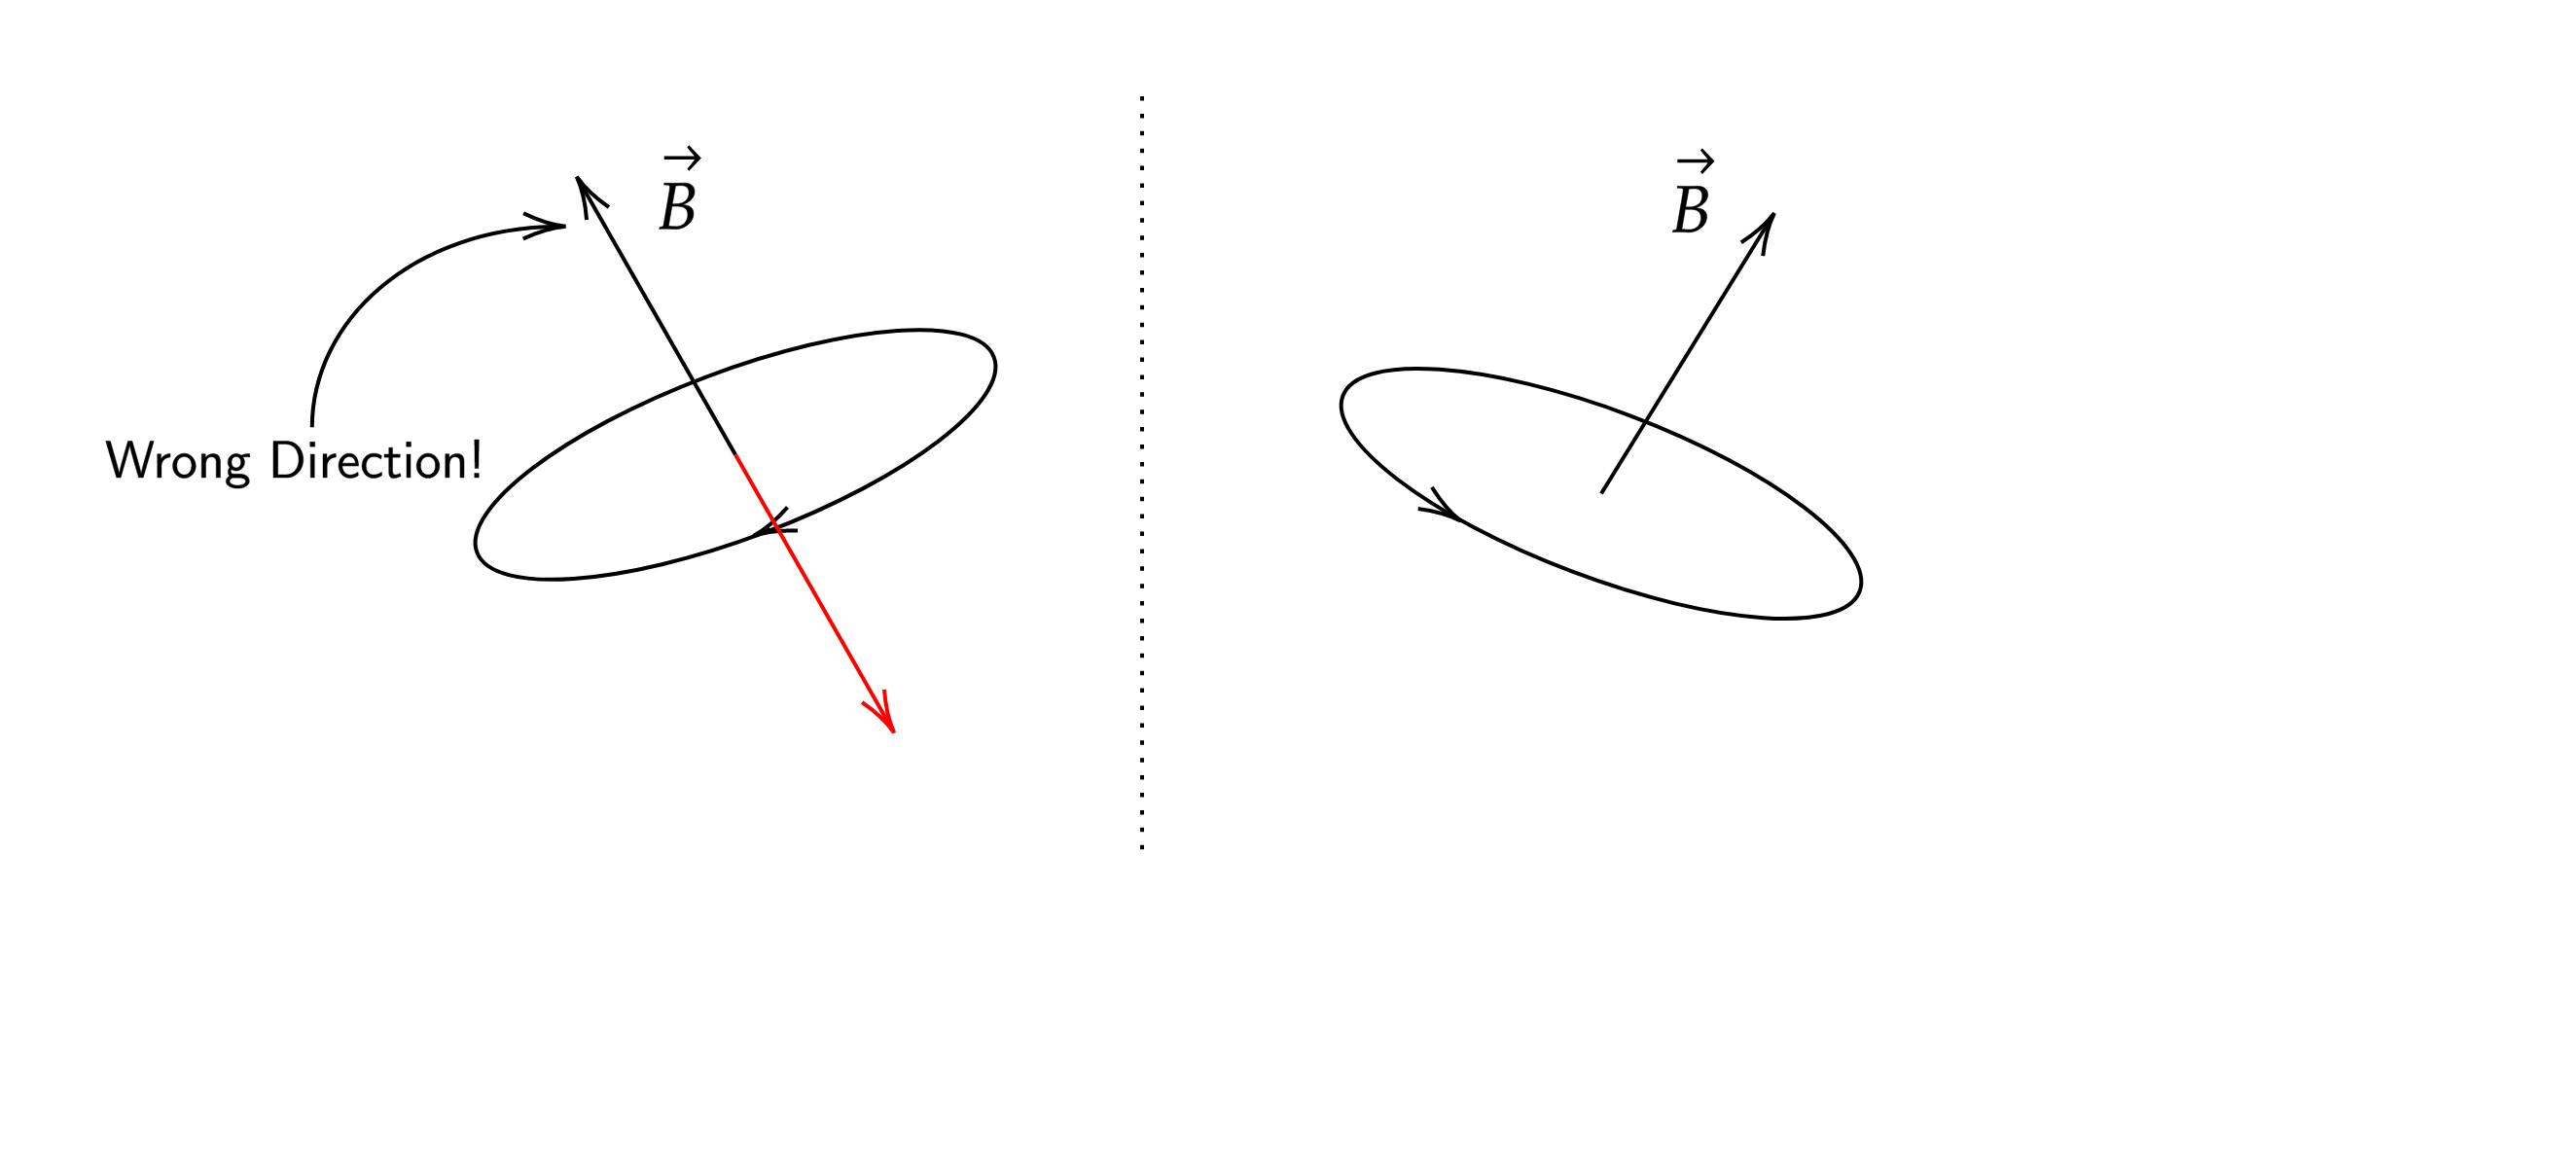
\includegraphics[scale=0.13]{Figures/BField.png}
\end{figure}
\end{frame}

\begin{frame}{The Physical Problem}

Quantities defined in terms of the cross product all suffer from this issue, and are thus called \emph{pseudovectors}.
\pause

Thus a mathematical construction is needed that defines these quantities rigorously while following sensible symmetries of physical systems.
\pause

This is achieved through the introduction of \alert{Geometric Algebra} also known as Clifford Algebra 
	
\end{frame}

\begin{frame}{Geometric Algebra}

Consider the orthonormal basis for the vector space $\mathbb{R}^3$, $\{\vb e_1, \vb e_2, \vb e_3\}$. Using this we can construct the \emph{inner} and \emph{exterior} products of combinations.

\pause

\begin{itemize}
	\item \only<4,5>{\alert{Symmetric}} Inner product maps two vectors to a scalar
	
	\begin{equation}
		\cdot : \mathbb{R}^3 \cross \mathbb{R}^3 \mapsto \mathbb{R}
	\end{equation}

	\pause
	\item \only<5>{\alert{Antisymmetric}} Exterior product maps two vectors to an element of a higher rank tensor product space
	
	\begin{equation}
		\wedge : \mathbb{R}^3 \cross \mathbb{R}^3 \mapsto \mathbb{R}^3 \otimes \mathbb{R}^3
	\end{equation}
\end{itemize}
\end{frame}


\begin{frame}{Geometric Algebra}
For some $a, b \in \mathbb{V}$, the object $a \cdot b$ is a scalar, which we will call grade 0 objects.
\pause

The object $a$ is a vector, which may be considered geometrically as an oriented line segment. We will call these grade 1 elements.
\pause

The object $a \wedge b$ is a \emph{bivector}, and may be considered as an oriented plane segment. We will call these grade 2 elements.
\end{frame}

\begin{frame}{Geometric Algebra}

\begin{figure}
	\centering
	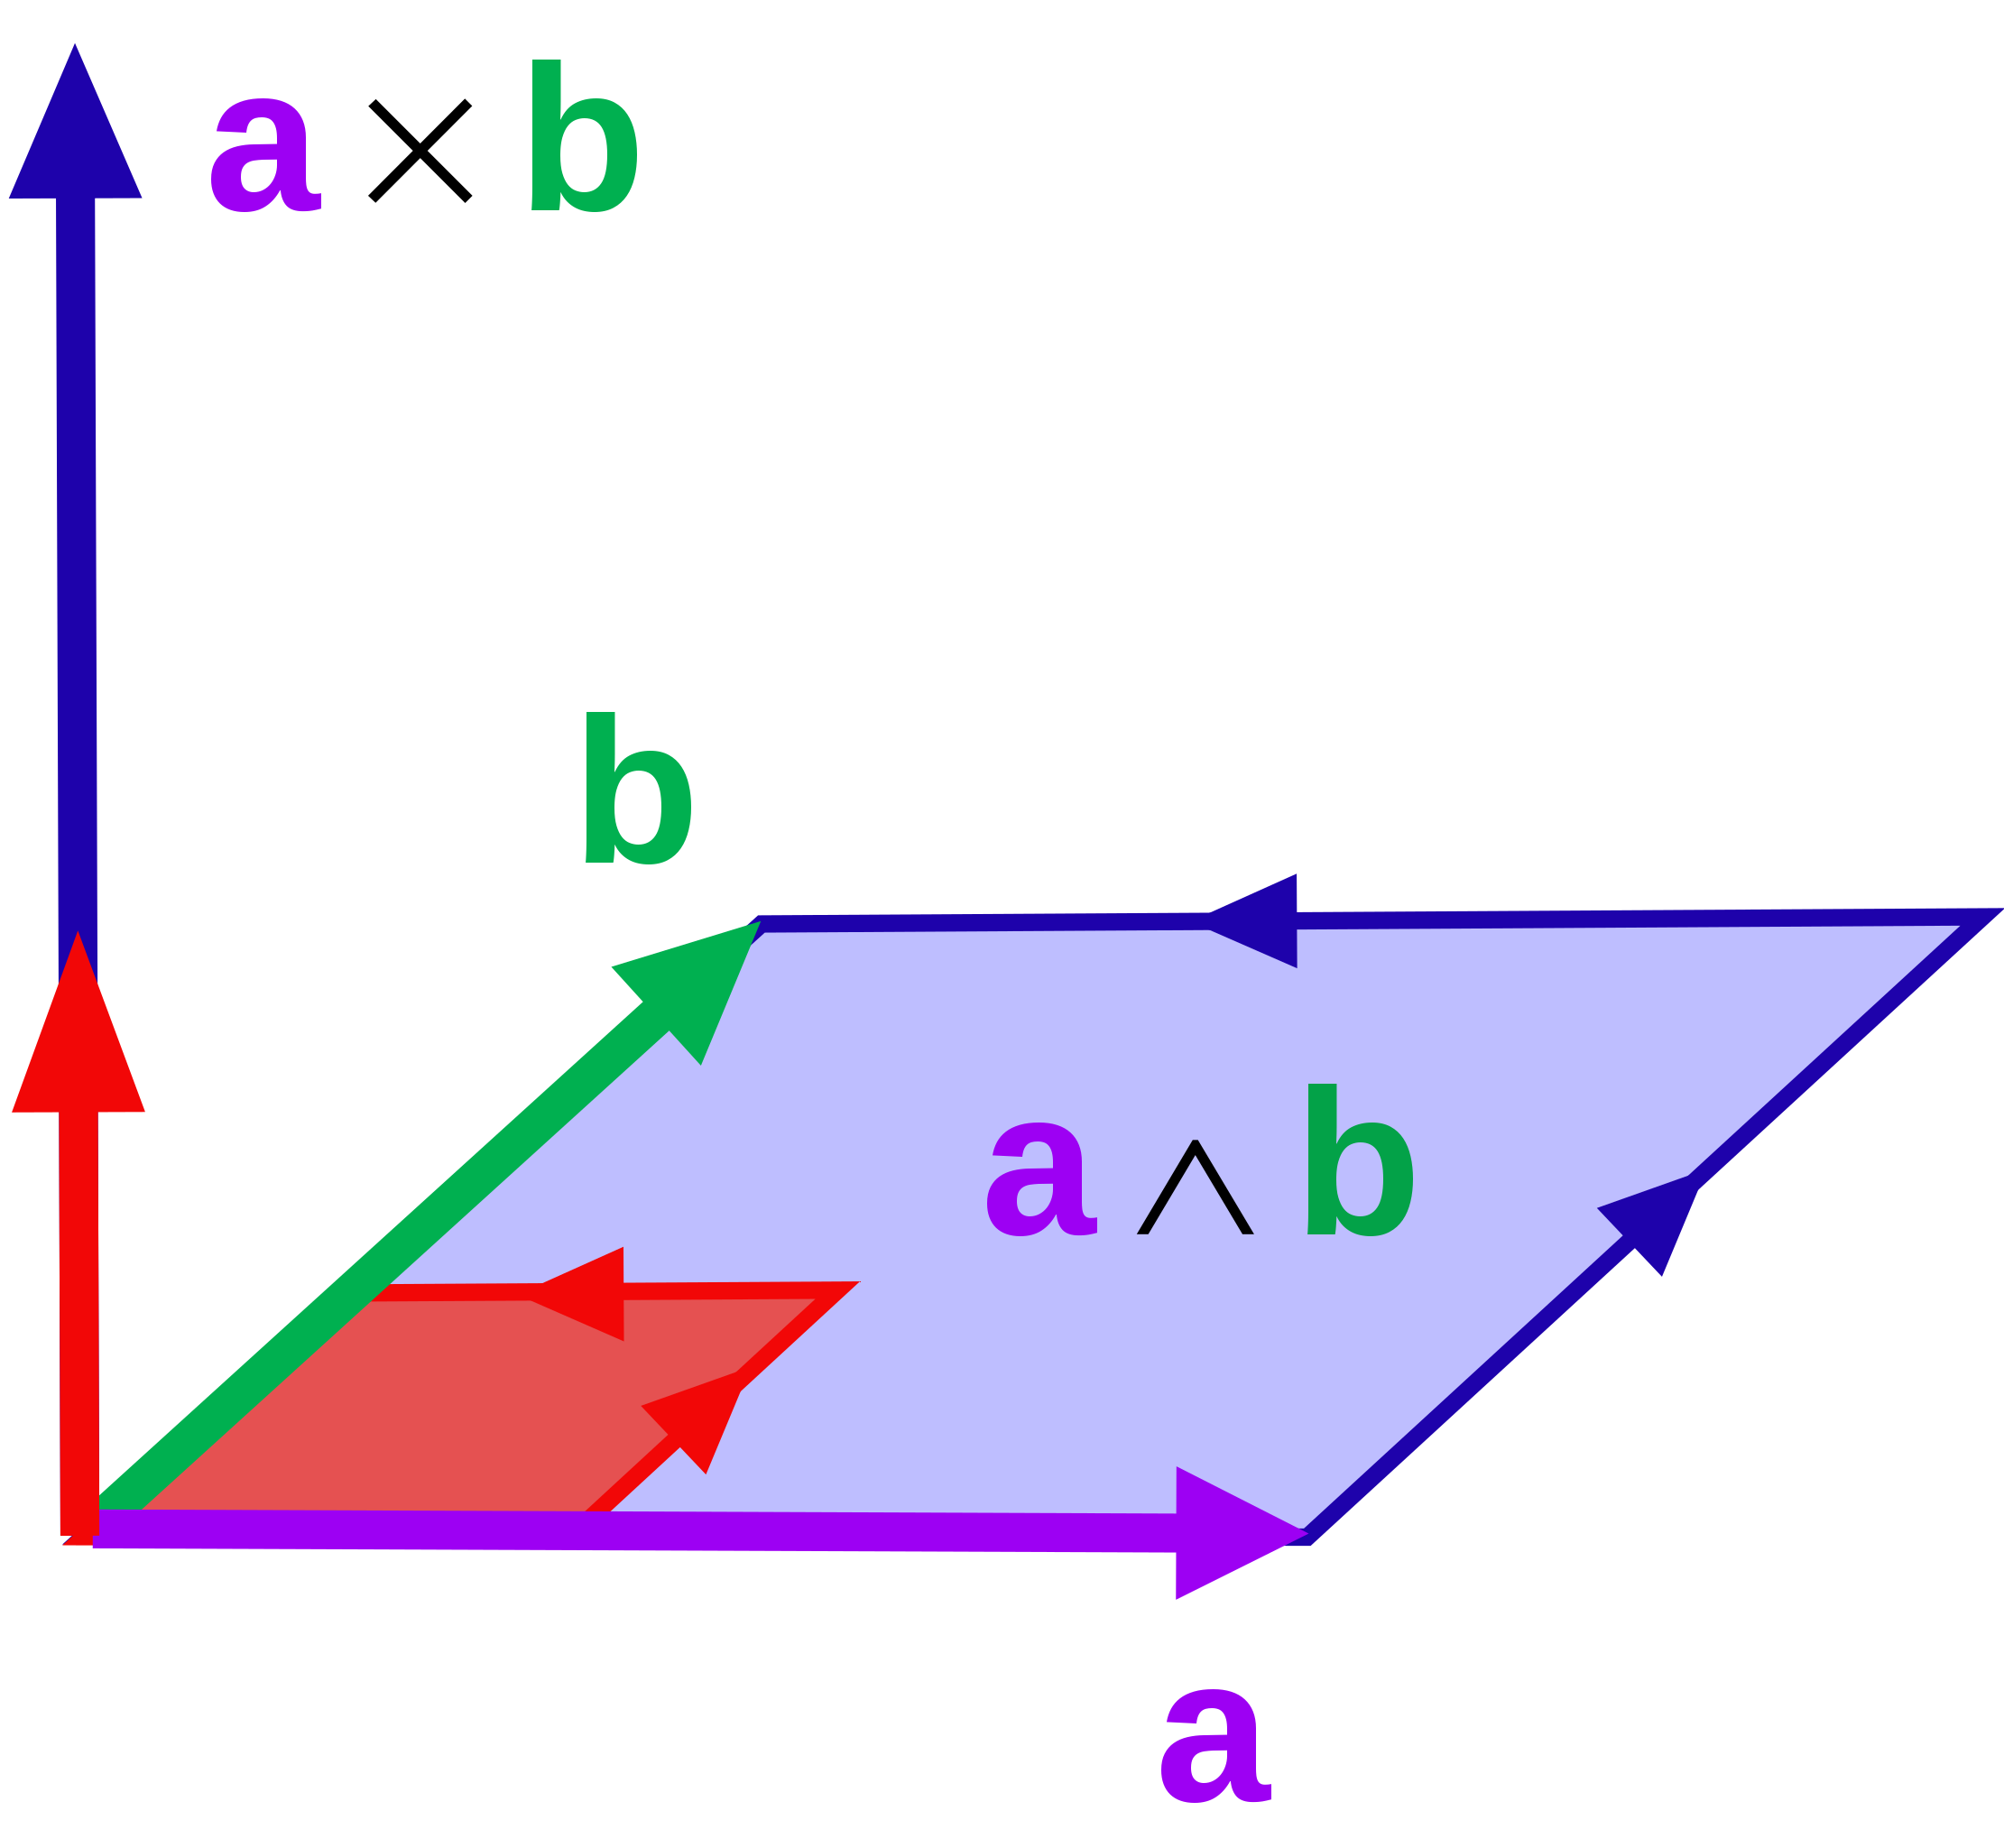
\includegraphics[scale=0.1]{Figures/Exterior_calc_cross_product.svg.png}
\end{figure}

\end{frame}

\begin{frame}
\frametitle{Geometric Algebra}

Using a combination of these we introduce a vector multiplication operation known as the \emph{geometric product} of vectors. For some  $a, b \in \mathbb{V}$, the geometric product of these vectors is

\begin{equation}
	ab = a \cdot b + a \wedge b
\end{equation}

\pause

This new construction does not return an element of the vector space, thus a new mathematical object is needed based on the elements of $\mathbb{V}$. \pause This object is the \emph{Clifford algebra of $\mathbb{V}$} denoted by $Cl(\mathbb{R}^3)$.

\end{frame}

\begin{frame}{Geometric Algebra}

To construct a basis for the Clifford algebra, we construct a basis of elements of every grade.
\pause

Exterior products are antisymmetric $\implies$ $a \wedge b = 0$ if $a$ and $b$ are linearly dependent. Thus the only possible basis elements are


\begin{table}
	\centering
	\begin{tabular}{c |c}
		\textbf{Grade} & \textbf{Basis}  \\
		\hline
		0 & 1 \\
		1 & $\vb e_1, \vb e_2, \vb e_3$ \\
		2 & $\vb e_1 \vb e_2, \vb e_1 \vb e_3, \vb e_2 \vb e_3$ \\
		3 & $\vb e_1 \vb e_2 \vb e_3$
	\end{tabular}
\end{table}

\pause

These form a \emph{tensor basis} for the Clifford algebra $Cl(\mathbb{R}^3)$ also known as \alert{The Pauli Algebra}.

\end{frame}

\begin{frame}{The Pauli Algebra}

The issues with the magnetic field and angular momentum arise due to their definition relying on the cross product. Only in 3 dimensions one finds a unique line orthogonal to a plane. \pause Thus a generalization of the cross product is required.

\pause

\only<3>{

Consider the vectors $\vb e_1$ and $\vb e_2$ and take their geometric product with the grade 3 trivector $\vb e_1 \vb e_2 \vb e_3$ -


\begin{align*}
	\vb e_1 \vb e_2 \vb e_1 \vb e_2 \vb e_3 &= - \vb e_1 \vb e_1 \vb e_2 \vb e_2 \vb e_3 \\
	&= - (\vb e_1 \cdot \vb e_1) (\vb e_2 \cdot \vb e_2) \vb e_3 \\
	&= -\vb e_3 \\
	&= -(\vb e_1 \cross \vb e_2)
\end{align*}
}

\pause

This pattern follows for all combinations, and thus we define the cross product as

\begin{equation}
	a \cross b \equiv -i(a\wedge b),
\end{equation}

where $i \equiv \vb e_1 \vb e_2 \vb e_3$ is the highest grade basis element.

\end{frame}

\begin{frame}{Hodge Duality}
\metroset{block=fill}
\begin{alertblock}{Hodge Duality}
	Multiplication by the highest grade element in an $n$ dimensional Clifford algebra induces a duality operation which maps grade $k$ elements to grade $n-k$ elements.
\end{alertblock}

\pause

In the 3 dimensional Pauli algebra, the cross product mappings are mappings from grade 2 elements ($a \wedge b$) to grade $3-2 = 1$ elements which are the orthogonal vectors produced by the cross product.

\pause

Vectors in a Clifford algebra have a multiplicative inverse defined as

\begin{equation}
	a^{-1} = \frac{a}{aa}.
\end{equation}

\end{frame}

\begin{frame}{The Gradient}
We can define a reciprocal basis given $\{\vb e_i\}$ as $\vb e^i = (\vb e_i)^{-1}$. The gradient is defined as

\begin{equation*}
	\grad = \vb e^i \partial_i
\end{equation*}
\pause

For a vector $\vb a$, the gradient can be decomposed as

\begin{equation*}
	\grad \vb a = \grad \cdot \vb a + \grad \wedge \vb a,
\end{equation*}

where $\grad \cdot \vb a$ is the \emph{divergence} and $\grad \wedge \vb a$ is the \emph{curl}.

\end{frame}

\subsection{The Dirac Algebra}

\begin{frame}{The Dirac Algebra}
The Pauli algebra is the algebra of 3 dimensional Equclidean space. The Dirac algebra is the algebra of 4 dimensional Minkowski spacetime.
\pause

Take a set of orthonormal basis elements $\{\gamma_0, \gamma_1, \gamma_2, \gamma_3\}$ of an inner product space $\mathbb{V}_4$. The metric signature is given by

\begin{equation*}
	\gamma_0\cdot\gamma_0 = 1 \qq{and} \gamma_k\cdot \gamma_j = -\delta_{kj}
\end{equation*}
Vectors that square to positive one are called \emph{timelike} and negative one are \emph{spacelike}.


\end{frame}

\begin{frame}{Spacetime Splits}
The Dirac algebra is a subalgebra of the Pauli algebra. This can be seen by constructing elements of the Dirac algebra that square to positive one, which will form the basis of the Pauli subalgebra.
\pause

Consider the elements $\gamma_k\gamma_0$ and take their square.

\begin{align*}
	\gamma_k\gamma_0\gamma_k\gamma_0 &= -\gamma_k^2 \gamma_0^2 \\
	&= - (-1) (1) = 1 = \vb e_k
\end{align*}

\pause

Thus timelike bivectors of the Dirac algebra are the vectors of the Pauli algebra.
\end{frame}

\begin{frame}{Spacetime Splits}

From this, we can see that for bivectors of the Pauli algebra we have

\begin{align*}
	\vb e_k \wedge \vb e_j &= \gamma_k\gamma_0 \wedge \gamma_j\gamma_0 \\
	&= -\gamma_k\gamma_j \gamma_0^2 \\
	&= -\gamma_k\gamma_j
\end{align*}

\pause

Thus, spacelike bivectors of the Dirac algebra form the bivectors of the Pauli algebra.

\pause

The scalars map to scalars and pseudoscalars map to pseudoscalars. Thus, by choosing a timelike vector, we can split all even graded elements of the Dirac algebra into the Pauli algebra.

\end{frame}

\begin{frame}{Spacetime Splits}

Vectors can also be decomposed into the Pauli algebra under multiplication by $\gamma_0$. We have for a Dirac vector $p$

\begin{align*}
	p\gamma_0 = p\cdot \gamma_0 + p\wedge \gamma_0
\end{align*}

We define $p_0 \equiv p \cdot \gamma_0$ and $\vb p = p \wedge \gamma_0$.

\end{frame}

\begin{frame}{The Dirac Gradient}

To finish the Dirac algebra, the gradient operator is defined similar to the Pauli gradient operator as

\begin{equation}
	\Box \equiv \gamma^\mu\partial_\mu
\end{equation}

\pause

The $\Box$ operator is itself a vector. Thus it can be split into a scalar and a Pauli vector by the choice of a timelike vector $\gamma_0$.

\begin{align*}
	\gamma_0\Box &= \gamma_0\cdot \Box + \gamma_0 \wedge \Box \\
	&= \partial_0 + \grad
\end{align*}

\end{frame}


\section{The Curvature Tensor}

\begin{frame}[allowframebreaks]{The Gradient, Revisited}

A set of four linearly independent vector fields at every point in spacetime define a frame at every point $\{\gamma_\mu\}$. This is called a \emph{frame field}.

The derivative in the direction of one of these vectors is denoted by $\Box_k$ and follows the following axioms.

\begin{enumerate}
	\item $\Box_\mu$ maps scalars to scalars $\Box_\mu \phi = \partial_\mu \phi$
	\item $\Box_\mu$ is a linear combination of partial derivatives.
	\item $\Box_\mu$ maps vectors to vectors. Any vector can be written as a linear combination of vectors a basis, and thus we have
	\begin{equation*}
		\Box_\mu\gamma_\nu = -L^\alpha_{\mu\nu}\gamma_\alpha,
	\end{equation*}
	where $L^\alpha_{\mu\nu}$ are the connection coefficients.
	\item $\Box_\mu$ obeys the Leibnitz rule
	\begin{equation*}
		\Box_\mu (A+B) = (\Box_\mu A)B + A(\Box_\mu B)
	\end{equation*}
	\item $\Box_\mu$ is a linear operator.
	\item $\Box_\mu$ transforms as a vector field.
\end{enumerate}

\end{frame}

\section{Maxwell's Equations}


\end{document}